\begin{frame}{Schweisshunde (Specialister i eftersøgning)}

\vspace{1em}

\begin{columns}[c] % c = center vertically

\column{0.05\textwidth} % Venstre margin

\column{0.7\textwidth} % Midten: Bullets

\small

\raggedright

\begin{itemize}

\itemsep0.6em % Justér afstand mellem bullets

\item Hundens opgave er udelukkende at \textbf{eftersøge anskudt/trafikeret vildt} (Schweiss = blod (tysk)).
\item De arbejder i et spor, der kan være \textbf{flere timer gammelt}, primært i line (sporsele).
\item Enhver jæger har pligt til at \textbf{tilkalde en schweisshundefører}, hvis de anskyder klovbærende vildt.
\item Hundene har en \textbf{trænet lugtesans} og et roligt temperament.
\item \textbf{Racer}: Hannoversk Schweisshund, Bayersk Bjergschweisshund, og i Danmark ofte Ruhåret/Korthåret Hønsehund (som er godkendt til opgaven).

\end{itemize}

\column{0.25\textwidth} % Højre: Ikon

\centering

\vspace{0pt}

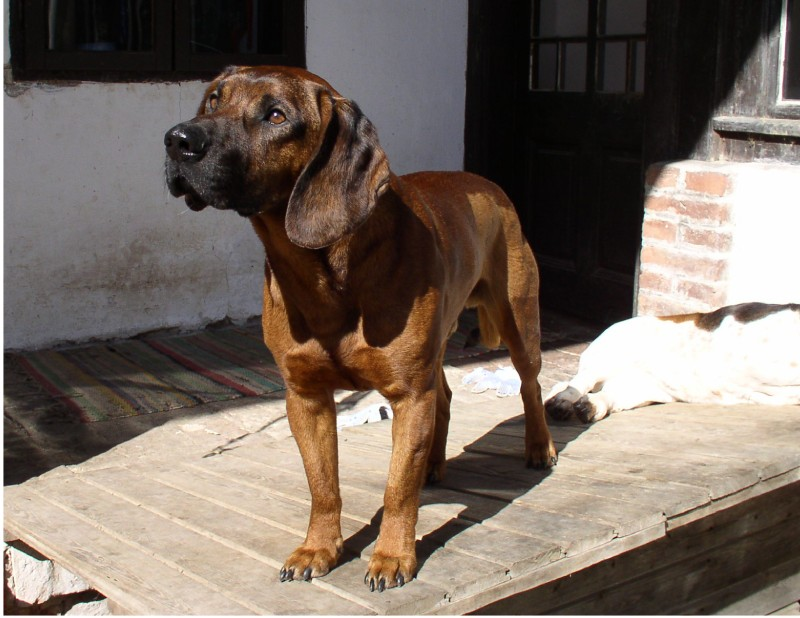
\includegraphics[width=0.9\linewidth]{Billeder/Jagthunde/schweisshunde/schweisshund.jpg} % Ikon af hund i sele/spor

\end{columns}

\end{frame}